%\documentclass[12pt, a4paper]{article}
%\documentclass[journal]{IEEEtran}
\documentclass[12pt, a4paper]{report}
%\documentclass{ActaOulu}

\usepackage{url}
\usepackage{refstyle}
\usepackage[hidelinks]{hyperref}

\usepackage{graphicx}
\usepackage{lscape}
% \usepackage{url}
% \usepackage{pdfpages}

\usepackage[backend=bibtex,style=authoryear]{biblatex}
% \usepackage{harvard}
\addbibresource{../cp.bib}

\begin{document}

\title{Project Proposal on\\
\bf{\textless Your project title\textgreater}}
\author{\textless Student Name\textgreater\\
\textless NCC ID\textgreater\\
Computing Project \\
Level 5 Diploma in Computing \\
% Email: email@email.com \\
Softwarica College of IT \& E-Commerce \\
Kathmandu, Nepal
}
\date{\textless Proposal submission date\textgreater}

\maketitle
\tableofcontents
% \listoffigures
% \listoftables
% \begin{abstract}
% This is abstract text: This simple document shows very basic features of \LaTeX{}.
% \end{abstract}
% \newpage

\chapter{Introduction} % (fold)
\label{cha:introduction}

This section sets the scene for your project.

What your project is about? Describe the domain of the project.

Provide overview of your project (may be with some diagrams!). Provide background and description of related concepts in your project.

If any external agency is involved you should explain what the agency is, why the project is required and any other relevant background.

What problem you are trying to solve? (Identity the domain problem)

Be systematic and elaborate in your problem identification section.

Why solving the identified problems matters? What benefits will the client/customer/user of your product have?

This should give reasons for the choice of this project, how the project draws on other modules of the course, what you hope (and expect) to gain from the project and other, similar aspects.

\section{Main features} % (fold)
\label{sec:main_features}

Give the list of main features that you want to have in your product. (give in bullets)
\begin{enumerate}
  \item View student marks for each exam
  \item Second feature
  \item Third feature
  \item ...
\end{enumerate}
What features will not be in your project? Why? (Write this only if necessary!)

Identify and list out your choice of programming languages, tools, development environments, platforms, and any other relevant technical aspects of your proposed project.

% A description of the technical challenges specific to the project will include items such as problem solving, applying analytical techniques, critically reviewing design decisions, or applying innovative thinking.
% section main_features (end)

\section{Aims} % (fold)
\label{sec:aims}

State one or two major goals/aims of your project.
for example:\\
\begin{itemize}
  \item To build desktop application for managing student information of ABC college
  \item To automate the student information management process in ABC college
\end{itemize}
% section aims (end)

\section{Objectives} % (fold)
\label{sec:objectives}
Objectives are the set of activities that you perform to achieve the stated aims. Your objectives should be SMART.

Some of the objectives will be technical(for instance, to solve some technical problem) and some will be personal (for instance, to learn a new programming language), and some academic (for instance, to learn different approaches to research activities).

State the objectives that you will have to perform to achieve the stated aim. For example:
\begin{itemize}
  \item To gather requirements from the stakeholders
  \item To design ...
  \item To develop ...
  \item To test ...
  \item To document ...
  \item ...
\end{itemize}
 % section objectives (end)

\section{Development methods} % (fold)
\label{sec:development_methods}
Describe which development method you choose and why?

Refer to NCC lecture notes for available types of software development methods. Choose either object-oriented or agile methodology.

You are suggested to use \emph{object-oriented} methodology.

Find your own reasons for selecting object-oriented methodology in your project (Look at advantages of \emph{rational unified process}). 
% section development_methods (end)
% chapter introduction (end)

\chapter{Project plan} % (fold)
\label{cha:project_plan}
Your project plan will be in this chapter. Describe how you are actually going to prepare and present the project plan here (tools used, and so on).

Give your readers directions about where they can find relevant information in this chapter.

\section{Work Breakdown Structure (WBS) and Time Estimate} % (fold)
\label{sec:work_breakdown_structure}
Describe what is the purpose of WBS in your project? How it will help in your project plan?

Your WBS should identify all of the project related activities you are actually going to perform in your project. Some high level activities that you actually going to perform are:
\begin{itemize}
  \item Proposal
  \item Analysis
  \item Design
  \item Implementation
  \item Testing
  \item Reporting
\end{itemize}

\begin{table}[htb!]
    \begin{center}
        \begin{tabular}{l|l|l}
        \textbf{WBS \#} & \textbf{Task name} & \textbf{Days} \\
        \hline

        \hline
        0. & \textbf{Your project name} & total\\
        \hline
        1 & \textbf{Project Management} & 15\\
        1.1 & Scoping & 5\\
        1.2 & Planning & 5\\
        1.3 & Monitoring \& Controlling & 5\\
        \hline
        2 & \textbf{Analysis} & -\\
        2.1 & Use cases & - \\
        2.2 & Requirements & - \\
        2.3 & Architecture & - \\
        \hline
        3 & \textbf{Design} & -\\
        3.1 & Structural model & -\\
        3.2 & Behavior model & -\\
        \hline
        4 & \textbf{Testing} & -\\
        4.1 & Unit testing & -\\
        4.2 & Integration testing & - \\
        \hline
        5 & \textbf{Reporting} & -\\
        5.1 & User manual & -\\
        5.2 & Final report & -\\
        5.3 & Presentation materials & -\\
        \hline

        \hline
        \end{tabular}
    \end{center}
    \caption{Example work breakdown structure with time estimate}
    \label{tab:wbs}
\end{table}

Adjust your estimation based on your final reporting deadline.

Build your own WBS for your project!
% section work_breakdown_structure (end)

\section{Milestones} % (fold)
\label{sec:milestones}
Identify at least 3 major milestones of your project with their planned delivery dates.
For example:
\begin{table}[htb!]
  \begin{center}
    \begin{tabular}{l|l}
    \textbf{Milestones} & \textbf{Date} \\
    \hline \hline
     Project proposal  & \date{July 4, 2014}\\
    \hline
      Analysis specification & \date{July 18, 2014}\\
    \hline
     Design specification & \date{August 8, 2014}\\
     \hline
     Final report & \date{September 15, 2014}\\
    \hline
    \end{tabular}
  \end{center}
  \caption{Milestones}
  \label{tab:milestones}
\end{table}
% section milestones (end)


\section{Schedule} % (fold)
\label{sec:schedule}

Describe how you scheduled your activities?

Your Gantt chart will be here Figure~\ref{fig:gantt}. Your Gantt chart should show milestones as well.

% \begin{landscape}
% \begin{figure}[htb!]
% \centering
%   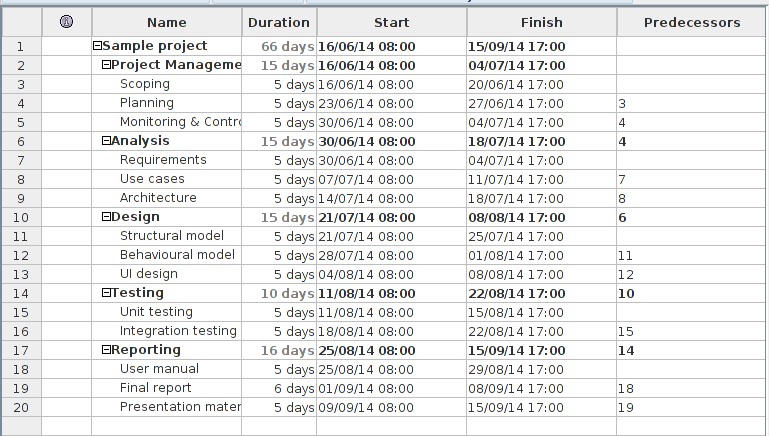
\includegraphics[width=9in, height=5in]{../img/sample_project_spread}
%   \caption{Spreadsheet of sample project}
%   \label{fig:spread}
% \end{figure}
% \end{landscape}

\begin{landscape}
\begin{figure}[htb!]
  \begin{center}
    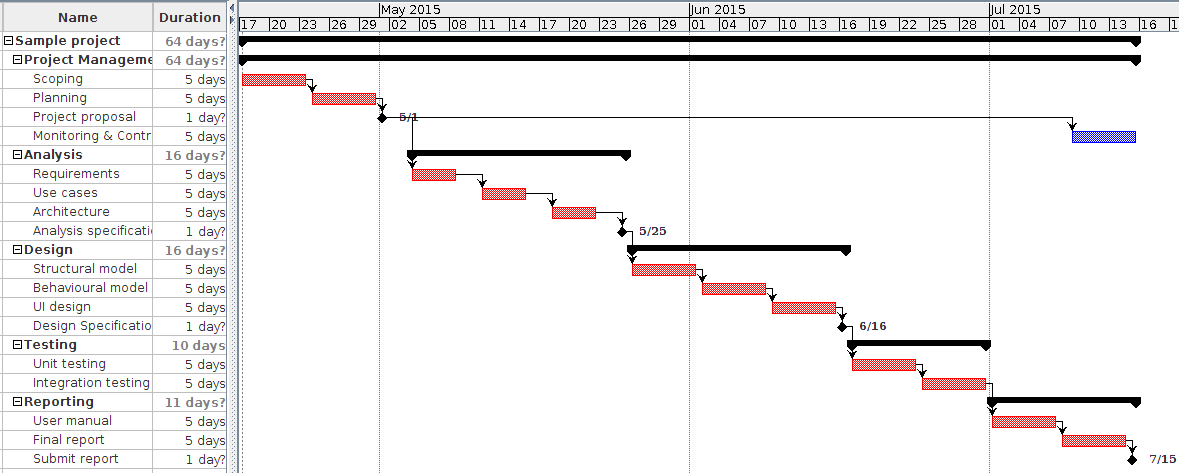
\includegraphics[width=9in, height=5in]{../img/sample_gantt.png}
  \end{center}
  \caption{Sample Gantt chart}
  \label{fig:gantt}
\end{figure}
\end{landscape}

% section schedule (end)
% chapter project_plan (end)

\chapter{Risk Management} % (fold)
\label{cha:risk_management}
Perform risk management in your project here! (Refer to lecture notes and the book)

To estimate the impact of each identified risks we use

\[
  Impact = Likelihood \times Consequence
 \]

relation. In this relation, the likelihood and consequence values are assigned based on the scale shown in Table~\ref{tab:likelihood} and Table~\ref{tab:consequence}.

You have to identify at least 5 risks for your project and suggest appropriate risk alleviation approach using tabular form as shown in Table~\ref{tab:risk_impact}. You have to provide the values table for likelihood and consequence as shown in relevant tables.

\begin{table}[htb!]
  \centering
\begin{tabular}{l|c}
  \bf{Likelihood} & \bf{Value}\\ \hline\hline
  Low & 1 \\ \hline
  Medium & 2 \\ \hline
  High & 3 \\ \hline
\end{tabular}
  \caption{Risk likelihood values (\cite{dawson2005projects})}
  \label{tab:likelihood}
\end{table}

\begin{table}[htb!]
  \centering
\begin{tabular}{l|c}
  \bf{Consequence} & \bf{Value} \\ \hline\hline
  Very low & 1 \\ \hline
  Low & 2 \\ \hline
  Medium & 3 \\ \hline
  High & 4 \\ \hline
  Very high & 5 \\ \hline
\end{tabular}
  \caption{Risk consequence values (\cite{dawson2005projects})}
  \label{tab:consequence}
\end{table}


\begin{table}[htb!]
	\centering
\begin{tabular}{l|c|c|c|p{4cm}}
	\bf{Risk} & \bf{Likelihood} &\bf{Consequence} &\bf{Impact} &\bf{Action}\\ \hline\hline
Hard disk crash & 2 & 4 & 8 & Investigate cost and prepare reliable backup\\ \hline
.. & .. & .. & .. \\ \hline
.. & .. & .. & ..\\ \hline
\end{tabular}
  \caption{Risk management sample table}
  \label{tab:risk_impact}
\end{table}
% chapter risk_management (end)

\chapter{Configuration Management} % (fold)
\label{cha:configuration_management}
Describe your configuration management plan here!. Configuration management is about managing and tracking various changes in your project's artifacts from inception to the final presentation. I suggest you to use \emph{Git}-- \url{https://git-scm.com/} to version control your project artifacts through out its life time. 

% Use a simple directory structure for configuration management! Refer to the configuration management approach discussed in the student's handbook!
% (short description!)
% You also have to show your directory structure as shown Figure~\ref{fig:dirtree}:

% \begin{figure}[htb!]
% \centering
%   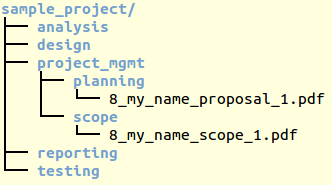
\includegraphics[]{../img/cm_sample}
%   \caption{A example directory structure for demo\_project}
%   \label{fig:dirtree}
% \end{figure}
% chapter configuration_management (end)

\chapter{Conclusion} % (fold)
\label{cha:conclusion}
Provide conclusion for your project proposal.
% chapter conclusion (end)

\printbibliography
\end{document}